%%%%%%%%%%%%%%%%%%%%%%%%%%%%%%%%%%%%%%%%%%%%%
% Template for Master and Bachelor theses   %
% at DSV, an adaptation made by Beatrice    %
% Åkerblom of the                           %
%%%%%%%%%%%%%%%%%%%%%%%%%%%%%%%%%%%%%%%%%%%%%
% Template for Doctoral Theses at Stockholm %
% University. The template is based on      %
% the layout an typography used in for      %
% dissertations in the Acta Univeristatis   %
% Upsaliensis series                        %
% Ver 3.0 SU - 2006-09-28                   %
%                                           %
% Erik Siira                                %
% erik.siira@ub.uu.se                       %
% Tel. 471 39 70                            %
%                                           %
% Special thanks to                         %
% Anders Källström,                         %
% Robert Nyqvist                            %
% and other studens who have used the       %
% former version of this template and       %
% submitted valuable feedback.              %
%%%%%%%%%%%%%%%%%%%%%%%%%%%%%%%%%%%%%%%%%%%%%


\documentclass[12pt,
               a4,
%               swedish,     % Uncomment this line if you write in Swedish
               twoside,
               openright]{book} % Default font 11pt, all pages are
                                % printed the same, new chapter always
                                % begins on a right-hand page.

% \usepackage[frame,a4,center]{crop} % Mount on A4 paper for preview
%% Use this (by uncommenting) if your printer complains that the paper
%% size is not A4.  Don't use it when the final version is produced.


% Package import
% Language, diacritics and hyphanation
               \usepackage[swedish,english]{babel} % Use English
                                                   % and Swedish
                                                   % languages. English
                                                   % default. English
                                                   % hyphenation.
               % \usepackage[latin1]{inputenc} % Unix users should
                                             % include this
                                             % package instead of
                                             % ansinew or applemac
                                             % for correct
                                             % handling of
                                             % diacritics.
              % \usepackage[applemac]{inputenc} % Macintosh users
                                                % should include this package 
                                                %instead of ansinew or latin1 
                                                %for correct handling of diacritics.
              %\usepackage[ansinew]{inputenc}  % Windows users include this package 
                                               %instead of applemac or latin1 for 
                                                %correct handling of diacritics. 
              \usepackage[utf8]{inputenc}
              % \usepackage{hyphenat}
\usepackage[T1]{fontenc}

% Page elements
\usepackage{mathptmx} % Default font for dissertations is Times.
%\usepackage{fourier} % If mathematics don't display well using
                      % Times, then use Fourier.
\usepackage{helvet}  

\usepackage{ThesisSU} % This package is specific for theses
                      % written at Stockholm University. 
                      % Modifications to the classfile and the 
                      % document can be found here.
%\ifpdf
%   \usepackage[pdftex]{graphicx}
%  \else
%    \usepackage[dvips]{graphicx}
%\fi % Used for figures

% need to use dvipdfm (current build order latex->bibtex->latex->latex->dvipdfm)
\usepackage{graphicx}
\graphicspath{{Figures/}}
\DeclareGraphicsExtensions{.eps}

% trying instead of below
 \usepackage{url}

%\usepackage[backref, colorlinks=true, urlcolor=black, pagecolor=black,
%linkcolor=black, citecolor=black, filecolor=black,
%menucolor=black, pdfpagelayout=TwoColumnRight, pdfstartview=FitH,
%plainpages=false,
%pdfpagelabels]{hyperref} % Use this package to obtain links in the
                         % electronic version of the document. All
                         % hyperlinks and other links
                         % should be black. Page view is set to
                         % Fit Width and page layout is set to
                         % display the document spread.  Make page
                         % anchors using the formatted form of the
                         % page number.  Set PDF page labels;
                         % i.e., write the value of \thepage to
                         % the PDF file so that Acrobat Reader can
                         % display the page number as (say) 'ii (4
                         % of 40)' rather than simply '4 of 40'.
                         
\usepackage{enumitem}
\setdescription{font=\normalfont\textit}

% Bibliographic information
% Filling in this bibliographic information facilitates the
% processing of this document.

% Insert linebreaks if necessary

% Just leave the posistion blank for any information that doesn't
% apply for your thesis, e.g. if your thesis doesn't have a subtitle:
%
% \newcommand{\thesisSubtitle}{}




% Abstract and titelpage

\firstAuthorFirstName{First}                % First author given name
\firstAuthorSurname{Author}                 % First author surname
\secondAuthorFirstName{Second}              % Second author given name
\secondAuthorSurname{Author}                % Second author given name

\firstAuthorEmail{email@dsv.su.se}              % First author's e-mail address
\secondAuthorEmail{email@dsv.su.se}             % Second author's e-mail address

\thesisTitle{Title of thesis}                   % The title of the thesis
\thesisSubtitle{Subtitle of the thesis, if any} % The subtitle of the thesis 

\thesisSubject{Computer and Systems Sciences}   % May be changed
                                                % to e.g. Human-Computer 
                                                % Interaction or other 
                                                % suitable for your thesis 
\thesisIsKind{Master}                           % Change to Bachelor if suitable
\theYear{2011}
\thesisCred{30}                                 % Change to 15 if Bachelor
\thesisAdvisor{Name of Advisor}
\thesisAssistantAdvisor{}                       % Name of Assistant Advisor,
                                                % if you have one
\thesisExternalAdvisor{}                        % Name of External Advisor,
                                                % if you have one

\thesisReviewer{Name of Reviewer}
\semester{Spring/Autumn}
\swedishTitle{Uppsatstitel}

                                               % The abstract text comes
                                               % here. Not more than 300
                                               % words. No empty lines.                                     
\abstracttext{ Qui terempri isuam liam incum aris forteat
  strudentre quid inculoc iviliaet; nihilius. Catimor demquam tam,
  senterf rmactum ompec orum, ne culvitimis se constusquam
  pratastiam porum rem, que poptert batia vidiem, sendum patus?
  Paturo vis esum inessus, furnimi iliciem ent vidit rebaturei
  potiu quam ductame teris, conductam me consum retis consuniu ma,
  speriam rem firisum publi, quam factod norehem et grat. Maesse,
  se orteliciemus cem.  Fuidena ilicien ervid C. M. C. me quid rem
  moente, conimus nit practanti, tabena, Ti. Habunterfer que
  avoltum quam hinaterniam abem nonside labistiae, intelic vidi
  ium erce enatici ecturox nulviribem hostio nesimoeritia rei
  inatis.}

\keywords{Keywords for the thesis, common in the domain.}




 % This file should be edited by the author.

\begin{document}
  
    \frontmatterDSV % Sets the frontmatter (Title page(s), abstract, keywords, etc.)
    
    \tableofcontents
    
    % Optional tables
%    \listoftables
%    \listoffigures
    
    %Part 1 - Introduction
    
    \chapter{Introduction}
    \label{chap:introduction}
    
    \section{Background}
    \label{sec:background}
    % \subsection{Enterprise Structure}
Large enterprises have traditionally implemented formal, centralized forms of organizational structure~\cite{pearlson2009}, such as hierarchical or matrix structures. In these structures, communication patterns, roles and decision rights are strictly defined. This allows for management to have a high degree of control over the enterprise and therefore enforce compliance with standards, procedures and policies which results in a highly stable enterprise. However, this comes at the expense of agility; it is difficult for these organizations to quickly adapt to a changing environment. While centralized structures were appropriate for the business environments of the past, modern business environments demand a high level of agility.

Common components of modern business environments include cooperation with different organizations,  rapidly changing business activities and processes, and a rapidly changing competitive landscape. In order to properly handle these components, a high level of enterprise agility is necessary. In centralized organizations, decisions need to be discussed at all levels of the hierarchy in order to obtain the appropriate justification and approval. This takes time; by the time a decision is made, it is often too late for it to be effective. In contrast, having decision making on the operational level allows for quick decisions that enables an organization to take advantage of opportunities quickly. More decentralized structures, such as networked organizations~\cite{pearlson2009}, are examples of this. It is important to note that a lack of rigidity and formal structure does not mean a lack of organization. It is still important for a decentralized enterprise to maintain order in its activities; this organization just needs to be based on an underlying decentralized structure instead of centralized one. Consequently, decentralized organizations need solutions to the same problems faced by centralized organizations -- such as business-IT alignment -- but the solutions need to be supportive of decentralization over centralization. 

On the organizational level, Enterprise Architecture (or EA) is a practice for creating an architecture for an enterprise. EA takes a holistic view of an enterprise in order to bring its many components (such as goals, strategies, information systems, and processes) into alignment with each other. Many different EA frameworks currently exist, for example The Open Group Architecture Framework (TOGAF)~\cite{togaf9.1} and the Zachman Framework~\cite{zachman}. 

All frameworks address one or more of the following three different aspects: the process of creating an enterprise architecture, how to describe enterprises architecture, and a description of how to actually implement the described architecture. Together, these three aspects form a solution to the problem of how to organize the components of an entire enterprise.

Enterprises are not alone in their trend towards decentralization. In the technical world, for example, peer-to-peer applications are becoming increasingly popular. Peer-to-peer applications follow an architecture in which peers communication directly to each other, without the need for a central server. These applications now exist in many different areas, such as file sharing \cite{bittorrent}, content distribution \cite{blizzard}, revision control \cite{progit}, and even as a digital currency ~\cite{bitcoin2008}. 



% \subsection{Goals}
% This thesis will have two primary goals. The first goal is to show that current EA techniques are inadequate for decentralized business environments. Assuming the first goal is met, the second goal is to determine principals from the field of distributed computing that can be used to form the basis for EA of the next generation. 



    \section{Problem}
    \label{sec:problem}    
    The problem of business-IT alignment is a relevant problem for all types of organizations, regardless of whether they have a centralized or decentralized structure. Solving it allows all components of an enterprise to operate together in a collaborative manner for the purpose of maximizing overall benefit to the enterprise. Enterprise Architecture frameworks outline a formal way in which to solve this problem. This thesis argues, however, that modern EA frameworks are primarily supportive of centralized organizations, and as such, have some shortcomings when applied in decentralized organizations. 

Many modern organizations are becoming increasingly decentralized in order to deal with increasingly dynamic business environments~\cite{fulk1995}. Modern EA frameworks and methodologies need to be able to handle these environments, and while they often can, rapidly changing business conditions have been identified as a critical problem in EA~\cite{kaisler2005ea,lucke2010critical}. In \cite[Ch. 1]{Bente2012}, situations were identified where ``EA fails to keep pace with the speed of change in modern business'' and ``companies that, despite having a fully institutionalized EA in place, were in a state close to paralysis''. In \cite{najafi2010kasra}, Najafi and Baraani state that a main challenge of existing EA frameworks is that they are ``[i]nflexible to perceive business changes or opportunities and then change appropriately to adapt and adopt these changes''.

Furthermore, current EA frameworks rely on some organizational properties that are becoming obsolete with progressive decentralization. For example, TOGAF~\cite[Ch. 47]{togaf9.1} suggests an approval process based on hierarchy, with an Architecture Board responsible for decision making; and FEA sets enterprise-wide standards to be followed by all through a set of common reference models~\cite{sessions2007}. For these reasons, ensuring the suitability of modern EA frameworks for  decentralized business environments--which are highly dynamic--is becoming increasingly relevant. 

This thesis addresses the problem of creating a suitable EA for decentralized organizations. The goal here is not to create a new EA framework, but rather to enhance existing ones through some guidelines or principles that increase their suitability for decentralized business environments.

An important part of this thesis project is to analyze the suitability of existing EA frameworks for decentralization. Therefore, the problem will be fully explicated--including a precise definition, problem motivation, and root cause analysis--in the results chapter, Section \ref{sec:exproblem}.

%%%%%%%%%%%%
%%%%%%%%%%%%
%~\cite{kaisler2005ea}
%rapidly changing business conditions have been identified as a critical problem in EA
%
%
%Rapidly changing conditions
%%%%%%%%%%%%%
%%%%%%%%%%%%%
%~\cite{}
%The embracing nature of an EA coupled with the constantly changing environment its management takes place in, gives rise to a number of severe challenges.
%%%%%%%%%%%%%
%%%%%%%%%%%%%
%~\cite{Bente2012}
%On the other hand, we encountered companies that, despite having a fully institutionalized EA in place, were in a state close to paralysis. The conglomerate of business, organizational, and technical dependencies had grown to a muddle that made reasonable changes impossible. 
%
%EA is supposed to prevent such failures— so why do they keep happening? 
%
%EA fails to keep pace with the speed of change in modern business.
%
%
%Sometimes the EA organization has an overly rigid approach to enforcing its own standards. Instead of discussing a sensible level of standardization with the IT crowd on the ground, enterprise architects invest their energy in political fights for IT standards that are irrelevant at best and that stall creativity at worst.
%
%In addition, if enterprise architects claim to be the only decision-making body in technical matters, there is a huge risk that they create a bottleneck. If decisions take ages due to pending strategic issues, imminent changes in the business model, and so forth, IT projects can be seriously delayed. The practical consequence is that projects deliberately circumvent the enterprise architects— for example, by choosing less suitable technologies not managed by the EA group.
%
%An IT landscape requires continuous evolution. Concentrating only on the operational aspects of IT will not be enough to meet future challenges. Both the innovations on the business side— new products, markets, and business models— and on the technology side, require a constant renewal. It is one of the core tasks of EA to plan and monitor this evolution.
%
%Our analysis of EA failures and shortcomings has revealed that EA needs to find its proper position in a complex and chaotic environment. The solution is not about eliminating chaos altogether. That would overstretch the meager powers of the EA or IT organization, or it could turn EA into an overly rigid control freak— just the other side of the coin.
%
%As we will see, the real issue is to balance chaos and order properly. The question is how to leverage chaos to increase orderliness.
%
%
%
%%%%%%%%%%%%%
    
    \section{Research Questions}
    \label{sec:resq}
    This thesis work seeks to answer the following general research question:
\begin{quoting}
\textit{Do existing EA frameworks need to be extended in order to support decentralized organizations?}
\end{quoting}

Due to the general nature of this research question, two more specific questions will answered in order to answer the overall question:
\begin{enumerate}
\item What aspects of existing EA frameworks support decentralized organizations? What aspects do not?
\label{req:1}
\item What are the principles of an EA framework that supports decentralized organizations?
\label{req:2}
\end{enumerate}

    
    \section{Goals}
    \label{sec:resq}
    The purpose of this thesis project is to contribute to the field of EA by improving it's support for decentralization. This is supported by two primary goals: The first goal is to demonstrate specific aspects of existing EA frameworks that are supportive and not supportive of decentralized organizations. The second goal is to contribute towards an EA framework supporting decentralization by design an artifact that overcomes a subset of the identified shortcomings.
    
    \section{Purpose}
    \label{sec:resq}
    \input{sections/Part1_Purpose.tex}
    
    \section{Limitations}
    \label{sec:resq}
    Due to time constraints, this thesis project is not able to address the entirety of the problem identified. Instead, only a subset of identified issues with EA will be addressed. 
    
    \section{Chapter Layout}
    \label{sec:resq}
    This paper is structured as follows:
\begin{description}
  \item[Chapter 2 - Extended Background] An extended background on decentralization in organizations and on three modern EA frameworks is presented here. Additionally, the related subjects of Enterprise Integration and Enterprise modeling are covered as related works. 
  \item[Chapter 3 - Method] This chapter contains: a justification for following design science; the chosen research methods and strategies along with reasons for these choices and a discussion of alternatives; how these methods and strategies are actually applied for this research; and lastly ethical considerations are covered. 
  \item[Chapter 4 - Results] This chapter contains: an explication of the problem with how the EA frameworks of TOGAF, Zachman, and FEA support decentralization; an explication of the problem with the case organization's support for EA; an outline of the solution artifact, which takes the form of guidelines (part of Johannesson and Perjon's method artifact type~\cite[Ch. 2.4]{johannessonPerjons2012}), and its accompanying requirements; the design of the artifact, which was performed with the aid of knowledge on peer-to-peer architectures; a demonstration of the artifact based on a case study; and an argumentative evaluation of the artifact through it's demonstration.
  \item[Chapter 5 - Conclusions \& Discussions] This chapter describes the primary conclusions drawn from the results, a discussion of the validity of the results, a discussion of ethical and societal consequences, and recommendations for future works. 
\end{description}
    
    % Part 2, Scientific Base
    
    \chapter{Extended Background}
    \label{chap:extendedBackgrounf}
    
    \section{Enterprise Architecture}
    \label{sec:ea}
    \input{sections/Part2_EA.tex}
    
    \section{Decentralization in Organizations}
    \label{sec:organizations}
    This section will first discuss the forms of organizational structure defined in the literature. Second, the (de)centralization of current organization and, as a consequence, their styles of IT governance will be explored. We conclude this section by underpinning the challenges organizations have to face due to their progressive decentralization.

\subsection{What is a Decentralized Organization?} 
 
An organization can be structured in many different ways. Sachdeva \cite{sachdeva1990} defines organizational structure as "... institutional arrangements and mechanisms for mobilizing human, physical, financial and information resources at all levels of the system..." According to Jacobides \cite{jacobides2007}, "Organizational structure provides the frames through which individuals see their world. Thus, the way each organization is structured shapes an ecology of different, distinct frames that exist at the level of the organizational subunit." 
%Nystrom and Starbuck \cite{nystrom1981} define organisational structure as the arrangement and interrelationship of component parts and positions in an organization.

There has been a lot of research on specific forms of organizational structure. Taxonomies of organization forms are defined in  \cite{mckelvey1982}, \cite{rich1992}.   \textit{Classic} and \textit{modern} types of organizational structure are often recognized.  Classic types include simple centralized organizations ~\cite{Mintzberg1979}, bureaucratic organizations \cite{mintzberg1981}, divisional structure and functional structure. Modern  types include matrix structure, flat organizations, adhocracy. New forms of organizational structure emerged recently: collaborative networks, virtual organizations and coopetition.

According to Robbins \cite{robbins1997}, organizational structure has three components: complexity, formalization and centralization.  Complexity refers to the degree to which activities within the organization are differentiated; Formalization refers to the degree to which work is standardized; Centralization refers to the degree to which decision making is concentrated at one point in the organization. 

Following Luthens \cite{luthans2006}, centralization and decentralization can be also defined according to three factors: geographical or territorial concentration or dispersion of operations; functions;  extent of concentration or delegation of decision making powers. In \cite{pearlson2009},  the following characteristics of centralization are defined: the allocation of decision rights,  the structure of communication lines and  the choice of forms of coordination.

In a centralized organization, all decision making authority would reside with a single, top-level authority. In a completely decentralized enterprise all members would have equal decision making rights. Here, hierarchy manages the inter-dependencies between the different subunits of organization and often makes direct interactions and communications unnecessary \cite{thompson1967}.  Decentralized organizations instead have less formalized communication lines~\cite{pearlson2009, ahuja1998network}, and more fluid, project oriented teams.~\cite{applegate1988}

Centralized organizations lean towards primarily vertical style of coordination~\cite{Bolman2008}, which is characterized by formal authority, standardization and rules in operations and in IT, and planning and control systems. Decentralized organizations lean towards lateral coordination characterized by meetings, task forces, coordinating roles, matrix structures, and networks~~\cite{Bolman2008}. 

Below, popular forms of organizations focusing on their degree of centralization will be considered. 

\subsection{Forms of Organizational Structure and Decentralization}

\subsubsection{Classic Organizational Structures}

Pearlson and Saunders offer a thorough description of a pure hierarchical organization structure~\cite{pearlson2009}: Except for the top level position, each position has one superior and zero or more subordinates. Decision rights and communication lines are strictly defined and work their way down from the top (i.e. the center). The scope of a position is specialized and strictly defined by your superior and one works in assigned teams. The primary benefit of a hierarchy is that the high levels of management have strict governance and control over the company. Hierarchical organization structures are suited for stable, certain environments. 

Hierarchical organizations can be subdivided into simple centralized and bureaucratic organizations:

In simple centralized organizations, both strategic planning and operational decision making authority belongs to one person at the top. This structure can be found in small and single-person-owned organizations with only two hierarchical levels. 

Bureaucratic organizations \cite{mintzberg1981} are characterized by multi-level hierarchical structure and use of standard methods and procedures for performing work. 

Hierarchical organizations generally divide their labor either in terms of function, a grouping of common activities, or in terms of division, a grouping based on output (product). Two organizational structures, divisional and functional, can be identified accordingly.

\subsubsection{Modern Organizational Structures}

Matrix structure is another popular style of organization structure~\cite{pearlson2009} that can be seen as a mixture of functional and divisional structures. In this form, individuals are assigned two or more supervisors covering different (usually product and functional) dimensions of the enterprise. Pearlson and Saunders state that matrix organization structures are suited for dynamic environments with lots of uncertainty, presumably because their authority structure allows them to cover multiple aspects when making decisions. However, like a hierarchical structure, a matrix structure is a rigid construct with strictly defined roles, communication lines and decision rights. Authority still comes from the top in a centralized manner, even though it becomes more distributed among matrix managers at the lower levels~\cite{pearlson2009}. 
%Consequently, matrix structures still may not be perfectly suited for uncertain, dynamic environments. 

%Applegate, Cash, and Mills~\cite{applegate1988} support this statement, as they describe hierarchical and matrix structures as rigidly structuring "communication, responsibility, and accountability to help reduce complexity and provide  stability". They furthermore state that both matrix and hierarchical structures have the effect of stifling creativity and preventing organizations from being able to adapt effectively to rapidly changing environments. 

Flat organization is a novel type of organizations where only one or maximum two hierarchical levels are defined (similarly to simple centralized organizations). For example, Valve Corporation, a software company in the video game industry released their handbook in 2012~\cite{valveHandbook}.  Unlike simple centralized organization described above, individual employees have complete freedom despite there being a president/founder at the top: Nobody reports to anyone, and everyone is free to work on whatever they want to. This is an example of high decentralization.

Adhocracy~\cite{applegate1988,pearlson2009}  aims to discard traditional hierarchies in favor of decentralized decision rights and flexible communication lines connecting the entire enterprise. Specifically, instead of hierarchies, an adhocracy has a rapidly changing set of project oriented groups that have decision making authority and other powers  \cite{robbins1997}. Mintzberg describes an adhocracy as "a loose, flexible, self-renewing organic form tied together mostly through lateral means"~\cite{Mintzberg1979}.  

\subsubsection{Post-Modern Organizational Structures}

New forms of organizational structure enabled uniquely by modern information and communication technologies  Internet emerged recently:  collaborative networks~\cite{Camarinha-Matos2005} and coopetitions~\cite{Bengtsson2000}.

%Network organizations are characterized by subcontracting  their business functions \cite{????};

Related to the idea of adhocracy, is the concept of collaborative networks (CN). Camarinha-Matos and Afsarmanesh define collaborative networks as being composed of ``a variety of entities (e.g., organizations and people) that are largely autonomous, geographically distributed, and heterogeneous in terms of their: operating environment, culture, social capital, and goals.''~\cite{Camarinha-Matos2005} Three common characteristics in various CNs are autonomy in the individual entities, a drive towards meeting common or complementing goals, and the use of an agreed-upon framework for collaboration. 

Under the umbrella of CNs, Camarinha-Matos and Afsarmanesh define virtual organizations, virtual communities, and virtual breeding environments~\cite{Camarinha-Matos2005}. Virtual organizations are a group of independent organizations working together to achieve some goal(s); virtual communities are communities of individuals that interact with each other through the use of computer network-based technologies; and virtual breeding environments are frameworks for interoperability set up by groups of organizations in order to enable the potential for forming a virtual organization.

%These entities collaborate through  computer networks in order to achieve common or complementary goals. The main driver behind CNs is that the goals the seek to achieve would be impossible or much more difficult to achieve without collaboration. %The composition of autonomous entities makes CNs a very relevant concept to decentralization. 

Another organizational form emerged recently is coopetition. Bengsston and Kock describe coopetition as a complex relationship between firms where they simultaneously compete and collaborate and benefit from both~\cite{Bengtsson2000}. Coopetition allows the participating organizations to take advantage of a heterogeneity of resources. Organizations may seek to create competitive advantage through a unique resource they own (e.g. skill). At the same time, it might be beneficial for them to cooperate with another organization that possesses a unique resource that is of value to them. 

Virtual organizations and coopetitions differ from the organizational structures defined above since they do not represent a single legal entity but a group of autonomous and independent entities with different (and possibly concurrent) strategic goals. These entities are engaged into collaboration in response to factors such as specific market situations, customer demand, etc.  The heterogeneous structure of such organizations remains invisible for a customer, while the service level agreements should be maintained at the same high level any other organization would maintain. Such organizational structures are grounded on a sustainable collaboration between partners without any centralized control.

%They explore the concept of coopetition in the context of competing firms that "produce and market the same product".~\cite{Bengtsson2000} In this context, they place an important limit on coopetition: their needs to be some kind of separation between the competing and cooperating aspects i.e. they can not "coopetate" in the same aspect. 

%An example of coopetition is Amazon.com's Marketplace; a platform provided by Amazon where any  competitor can list items for sale alongside Amazon's own sales, often of the same items~\cite{UnknownAskIrina,Amazon.com}. This allows sellers to take advantage of Amazon's platform while Amazon takes advantage of the increase in traffic. 

\subsubsection{Decentralization in Organizational IT}
According to Rockart et al.\cite{Rockart1996}, changes in business and technology as well as progressive decentralization of organization as a whole drives the changes in roles and structure  of IT units. The works presented in \cite{fulk1995, osterloh2000, Rockart1996, Weill2004} focus on the relation between the structure of an organization and its IT. 

Fulk \cite{fulk1995} discusses the interplay between communication technology and various organizational forms. The authors consider communication technologies as one of the key enablers of inter-organizational and intra-organizational changes.

In \cite{osterloh2000}, authors study how different organizational forms affect the knowledge transfer in organization. They claim that ``Organizational forms enable different kinds of motivation and have different capacities to generate and transfer tacit knowledge.''

Weill~\cite{Weill2004} defines six forms of organizational structures in IT (called IT Governance archetypes) based on how the five major IT decisions in organizations are made. These archetypes are: business monarchy, IT monarchy, feudal, federal, IT duopoly and anarchy.   In a \textit{business monarchy} all IT related decisions are made in a centralized manner by the top-level executives (e.g. the CxOs). In an \textit{IT monarchy}, a group of IT professionals are responsible for making the decisions. This is also highly centralized as the authority resides with this group. An \textit{IT duopoly} is characterized by two groups, one of IT executives and the other of business executives, coming to agreements in order to make decisions. This is more centralized than the federal form, as the decisions are only made by the two groups, rather than each individual business unit having input. The \textit{feudal} is much less centralized. It is where individual organizational units are responsible for their own decisions. \textit{Federal IT  }would aim to balance these through a combination of central IT and IT in the business units. \textit{Anarchy} is a highly decentralized style of governance. It is similar to the feudal archetype, however the size of the units is much smaller. Instead of being an entire business unit, small teams or even individuals are responsible for their own decisions.

%This allows for systems that meet the individual business units needs, as well as enabling interoperability throughout the enterprise. 



%\subsection{IT Governance}

%\cite{Rockart1996} Some key weaknesses of centralized IT to eliminate are slow responsiveness and having systems that do not fit the needs of individual business units. Decentralized IT on the other hand lacks "synergy and integration"~\cite{Rockart1996} due to a lack of standardization.

% CAN GO TO THE SOLUTION PART? Federal IT would aim to balance these through a combination of central IT and IT in the business units. A primary task of the central IT would be to maintain standards for the entire enterprise. The business units would still have ownership of many of their own systems, allowing them to implement them as they deem best. This allows for systems that meet the individual business units needs, as well as enabling interoperability throughout the enterprise. 
%
%
%\begin{figure}
%\centering
%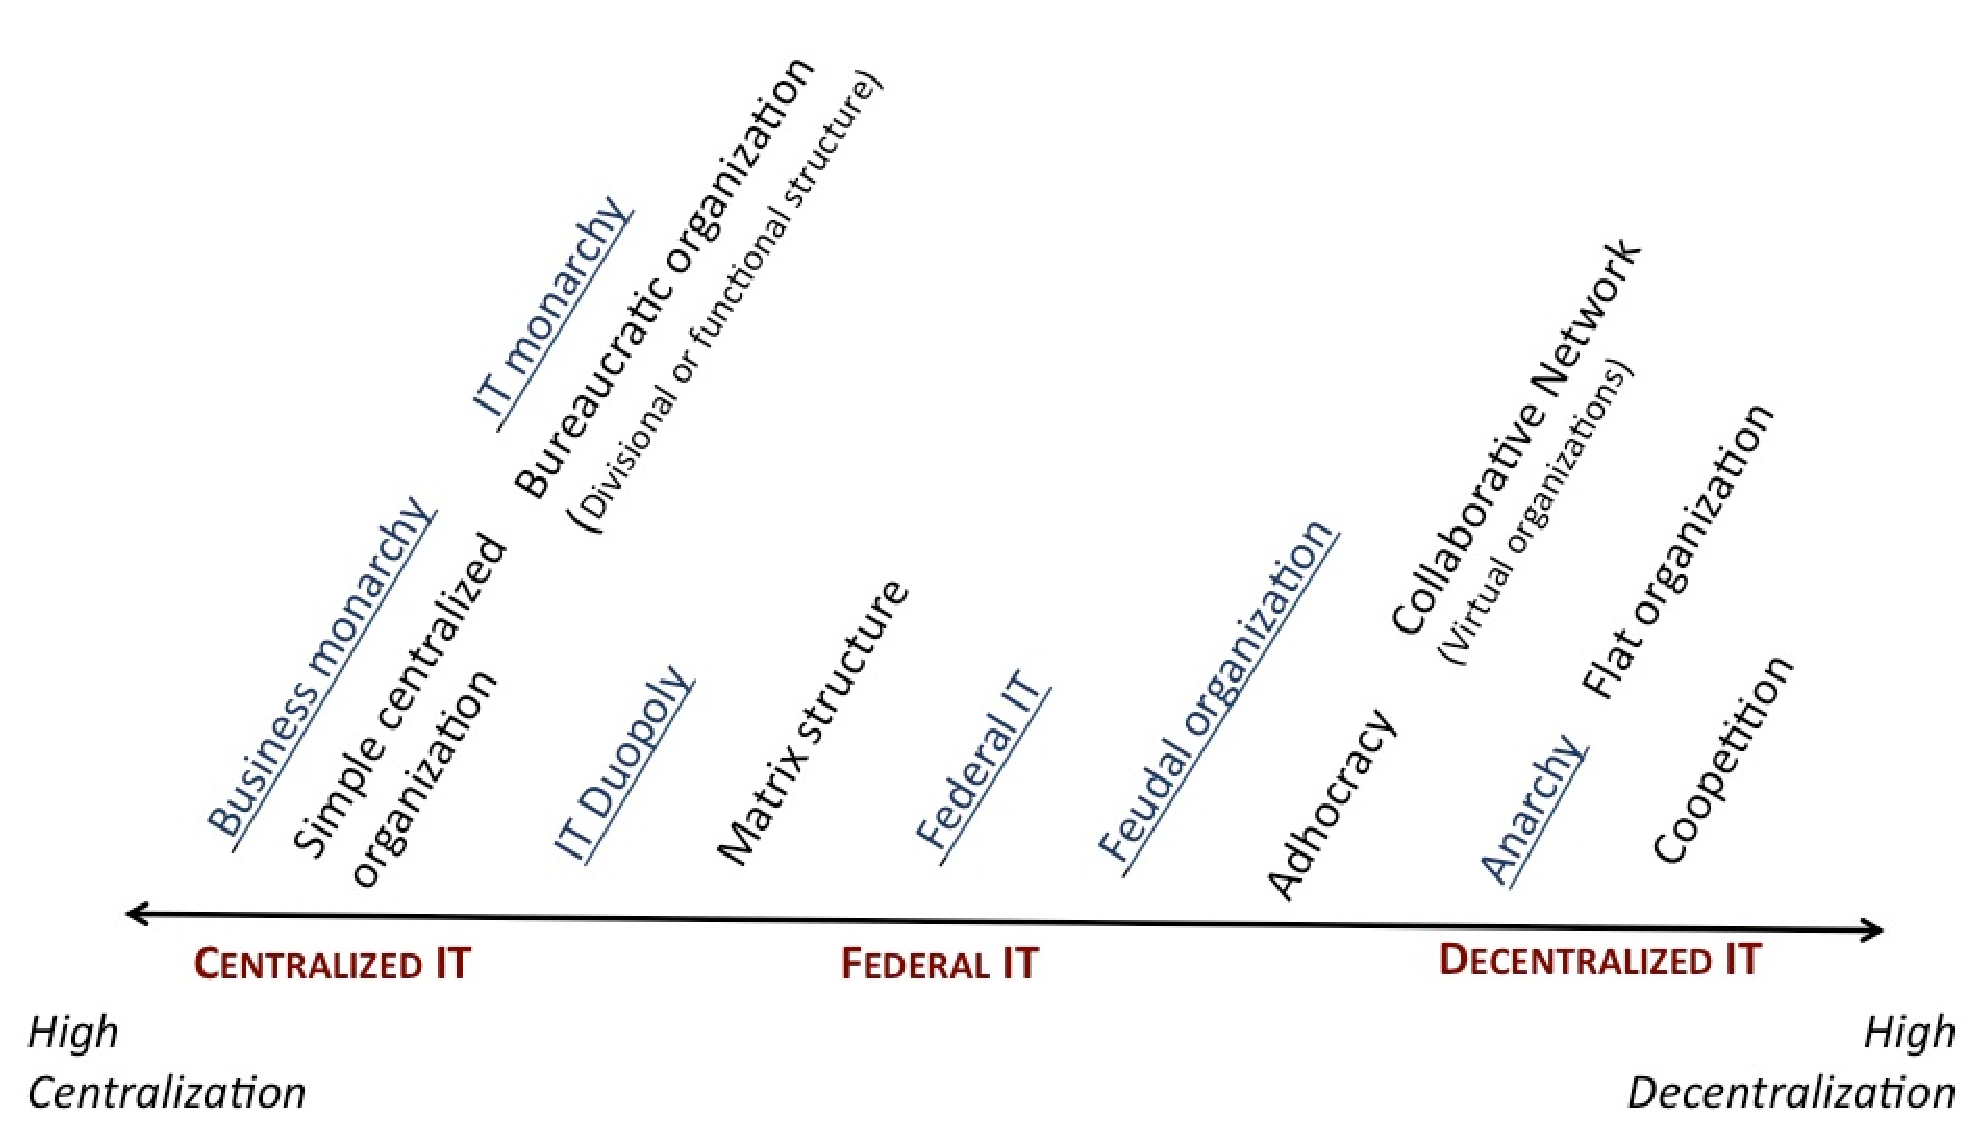
\includegraphics[scale=0.3]{taxonomy}
%\caption{Organizational taxonomy: From Centralized to Decentralized}
%\label{fig:taxonomy}
%\end{figure}

\subsection{Challenges of Progressive Decentralization in Organizational IT}
\label{sec:challenge}

%The trend appears to be moving away from the paradigm within which organizations strive for mass production efficiencies, hierarchical organization, and bureaucratic structures that provide central control over activities divided into small parts. The new paradigms may have as their premise the needed for flexible, learning organizations that continuously change and solve problems through interconnected coordinated self-organizing processes.

%From: Daft, Richard L., and Arie Y. Lewin. "Where are the theories for the" new" organizational forms? An editorial essay." Organization Science 4.4 (1993): i-vi.

%********

Modern organizational structures show a strong tendency towards decentralization \cite{daft1993} which results in changes to their management and operation styles. This heavily involves IT and requires major changes in organization processes. This transformation is not a mere question of ``flattening'' the organization by shifting authorities and decision making power from top to bottom hierarchical levels or from one person to a group. In classic organizations, not only does hierarchy ensure control and coordination, it also manages interdependencies between  different subunits of an organization which often makes direct interaction and communication unnecessary \cite{thompson1967}. As a result, a challenge related to decentralization and a ``weakened hierarchy'' is a lack of interaction and communication between organizational subunits. Another major risk of IT decentralization, according to \cite{Rockart1996}, is poor synergy and integration due to a lack of standardization.

Caruso, Rogers and Bazerman~\cite{caruso2008boundaries} highlight the importance of information sharing and coordination for these organizations. In order to succeed at these aspects, they outline three barriers that decentralized organizations need to overcome. The first barrier is intergroup bias; the tendency to treat one's own group better than other groups. The second barrier is group territoriality; the tendency for a group to protect their territory (physical or informational). The third barrier is poor negotiation strategies used by different groups when interacting with one another. 

Intergroup bias is direct result of having separate, autonomous groups within an enterprise~\cite{caruso2008boundaries}. The individual groups have a tendency to promote their own group over other groups, especially in situations where they are competing for a resource, such as a portion of the budget. A certain level of competition can be beneficial, however if it leads to hostility or distrust between groups, this can have a detrimental effect on their ability to share information and collaborate. This can prevent the groups from taking advantage of situations where they have to ability to work together for the benefit of everyone. 

The second barrier identified by Caruso et al. is group territoriality~\cite{caruso2008boundaries}. Group territoriality is characterized by group members taking action in order to protect their perceived territory. This can include physical territory such as space or tangible resources, as well as intangible territory, such as roles or information. Group territoriality is supported by a group's need to maintain its identity, its reputation of competence and sense of value, and a group's need for a stable home within the organization from which they interact with the rest of it. Group territoriality encourages ``a sense of psychological ownership''~\cite{caruso2008boundaries} for a group's members which can enforce the belief that they are the sole responsible party for a role or specific knowledge. This "inward-looking" behavior works against collaboration and information sharing. On the other hand, group territoriality can be beneficial; it can foster a sense of security in its members that ``facilitates planning and execution of activities''~\cite{caruso2008boundaries}. 

The third barrier identified by Caruso et al. in decentralized organizations is related to negotiations between groups, and how these negotiations are often conducted using ``poor negotiation  strategies''~\cite{caruso2008boundaries}. These poor strategies are the result of three common errors made while negotiating. The first error is a false belief in a ``fixed pie'' of value that is to be divided when negotiating. This prevents negotiating parties from recognizing situations where they are able to help each other, and therefore increase the size of the figurative pie. The second error is a failure to properly consider the other group's perspective. Understanding the other group's decision process, valuing process, and interests is key to discovering opportunities for helping one another, and the organization as a whole. The third error is when groups fail to even recognize they are in the process of negotiating. Instead, they see it as a competitive or hostile behavior where, again, they only see a fixed pie that is to be split up. This also prevents groups from taking advantage of opportunities to increase the size of the pie.    



   
    
    \section{Related Works}
    \label{sec:related}
    The practice of EA is just one potential solution to the problems of business-IT alignment. EA is a ``heavy-weight'' approach in that it aims to be a complete solution. However, other ``light-weight'' solutions do exist that focus on specific aspects of business-IT alignment and this section will briefly outline one of them: enterprise modeling.
  
%\subsection{Enterprise Modeling}

``Enterprise Modeling is the art of externalizing enterprise knowledge which adds value to the enterprise or needs to be shared. It consists in making models of the structure, behavior and organization of the enterprise''~\cite{Vernadat200215}. Through modeling, practitioners aim to better understand the current or future organization and function an enterprise. To this end, common enterprise categories of enterprise modeling include goal, process and value modeling. 

\paragraph*{Goal Modeling}

Goal modeling aims to describe the goals of an enterprise, their interrelations, means for achieving these goals, and additional factors that impact them. A specific example of a goal modeling technique is the Business Motivation Model (BMM)~\cite{bmm2010}. In BMM, means, ends and influencers of an organization are modeled and assessed. Here, the focus is on understanding what an organization wants to achieve (i.e. goals). The relationship between an organizations goals and its means is described, though the specifics of the means are not. 
%An EA, on the other hand, might use goal models, but if so, would use them as part of a bigger whole. This is in contrast with EA which takes a holistic approach in describing an entire enterprise, not only its goals.

\paragraph*{Process Modeling}

According to Roshen, ``[a] business process is a collection of related, structured activities or tasks that produces a specific product''~\cite{roshen2009soa}. Business processes are a complicated matter, and as such, process modeling is used to describe them in a detailed and accurate manner, in order to understand how an organization creates some output. Many different modeling languages exist, for example, Business Process Model and Notation (BPMN)~\cite{model2011notation}, Event-driven Process Chain (EPC)~\cite[Ch. 6]{scheer2005process}, and UML Activity Diagrams~\cite{uml241}. Processes can exist within an organization (intraorganizational) or they can interact with processes from other organizations (interorganizational). According to Weske~\cite{weske2012business}, ``the primary focus of intraorganizational business processes is the streamlining of the internal processes by eliminating activities that do not provide value''. Interorganizational processes, on the other hand, aim to specify and streamline interactions with other organizations. 

\paragraph*{Business Value Modeling}

Business value modeling depicts the exchange of value between entities. Examples of value modeling languages are e3 Value~\cite{Gordijn2001e3value} and REA~\cite{pavel2006model}. Business value modeling is used to understand what an organization does in order to create value. This allows it to be used as a starting point for the exploration of business ideas, design of processes, or development of systems~\cite{johannesson2011lecture}.

\paragraph*{Holistic Approaches}

A holistic approach to enterprise modeling can also be taken, where a combination of modeling techniques are used to represent an entire enterprise. The relationships between different models are specified, and a method for making the models may also exist. An example of a holistic modeling technique is Enterprise Knowledge Development (EKD)~\cite{stirna2007ten,bubenko2001user}, where an organization is modeled using six different models, each with a different focus. EKD also specifies a process for creating the models. A holistic approach to enterprise modeling such as EKD is similar to EA in that it specifies a process (similar to the EA method) and set of models that represent an enterprise (similar to EA description). However it is also quite different from EA in that it does cover how to transform those models into actual enterprise change.

%
%\subsection{Enterprise Integration}
%
%According to Vernadat, ``Enterprise Integration (EI) consists in breaking down organizational barriers to improve synergy within the enterprise so that business goals are achieved in a more productive and efficient way''~\cite{Vernadat200215}. To accomplish this, Vernadat states that EI relies ``free but controlled flow of information and knowledge, and the coordination of actions''. To this end, three general perspectives on EI exist: information-oriented, service-oriented, and process-oriented~\cite{zdravkovic2012}.
%
%Information-oriented integration is aimed at the integration of data. Two key components of information-oriented integration are standardizing how data is represented and enabling efficient access to it throughout an enterprise. Typical approaches to this are: data warehousing~\cite{kimball2006data}, where data from across the enterprise is consolidated to a single data warehouse in batches; data federation~\cite{haas2002data}, where a single system is used to query multiple data sources; and data replication~\cite{wiesmann2000database}, where data is copied between data sources at regular intervals. 
%
%Service-oriented integration is aimed the integration of functionality. The dominant architecture for service-oriented integration is Service-Oriented Architecture (SOA). Here, functionality is organized into services--worked performed by one application for another application--which have the characteristics of  reusability and composability~\cite{roshen2009soa}. These characteristics are important as they allow for services to be shared across and between enterprises (reusability), and for multiple services to be used together to create a new service (composability). 
%
%Process-oriented integration uses enterprise knowledge in conjunction with systems knowledge in order to integrate on the business process level~\cite{Vernadat200215}. Process-oriented integration builds on service-oriented integration in order to automate and order services for the production of some product. This can be done in both intra- and interorganization contexts, and is accomplished with the use of process models and systems dedicated to process management~\cite{dumas2005process}. A key advantage of process integration is that it provides a basis for communication between the IT and business sides of an enterprise~\cite{dumas2005process}.
    
    % Part 3 - Method    
    
    \chapter{Method}
    \label{chap:method}
    %Choice of research method:
%
%Description: Requirement for 1 point: that the choice of a research strategy and research methods is clearly motivated and described, that alternative research strategies and methods that could be used to solve the research question are discussed, as well as that relevant ethical considerations are discussed. For 2 points the following is also required: that alternative, applicable research strategies and methods are comprehensively discussed and that a profound reasoning about the chosen strategies and methods is made, where the motives for choices made are clearly evident. For 3 points the following is also required: that the choice of method is discussed in relation to the research strategies and methods that are used in current, related research studies that can be regarded as state-of-the-art.
%
%Instructions: It should be evident how the thesis relates to empirical and design research. If the thesis relates to design research then some method framework should be discussed, see for example A Design Science Primer. Research strategies, data collection methods, and data analysis methods should be described. See for example The Good Research Guide for the differences between theses. The description should include references to method literature. There should also be references to literature regarding ethical aspects, for example Appendix 1 in The Good Research Guide. The discussion should be closely tied to the research question of the thesis. There should not be long, general descriptions of research strategies and methods that are only summations from method literature without connections to the thesis topic.
%
%
%
%Application of research method:
%
%Description: Requirement for 1 point: that the application of the chosen scientific strategies and methods are clearly described and that relevant ethical aspects are discussed. For 2 points the following is also required: that the application of research strategies and methods are done in accordance to the demands of said methods and strategies and that a clear argumentation exists for this. For 3 points the following is also required: that there is a real depth to the data analysis
%
%Instructions: How the chosen research strategies and methods (both data collection and data analysis methods) were applied should be clearly described. If the thesis uses design research it should explain how the chosen method framework for design research has been applied. The description should include references to method literature. There should even be references to literature regarding ethical aspects, for example Appendix 1 in The Good Research Guide.



\section{Choice of Research Method}

Empirical research ``aims at describing, explaining and predicting the world''~\cite[Ch. 1]{johannessonPerjons2012}. In comparison, design research additionally wants to improve upon the world through the development of artifacts. This thesis project aims to improve EA by proposing an artifact that can extend the support of existing EA frameworks for decentralization. As a result, a design research approach, specifically design science, will be utilized. The remainder of this section seeks to further demonstrate the suitability of design science and outline the specific research strategies and methods chosen. 

\subsection{Design Science and its Relevance to this Thesis Work}

Design science is concerned with the development and application of \textit{artifacts} aimed at solving some practical problem~\cite{hevner2004,johannessonPerjons2012} in a manner that is of general interest~\cite[Ch. 1]{johannessonPerjons2012}. 

In order to be relevant, Design Science must exist in some context. Johannesson and Perjons~\cite[Ch. 1]{johannessonPerjons2012} define a generic context for design science in terms of people, practices and problems. A practice is a set of related activities performed regularly by people. In the performance of a practice, people encounter practical problems. Two general kinds of problems exist; one where the current state of affairs problematic and the desirable state is neutral, and a second where the current state is neutral and the desirable state is an improvement. The artifacts created through design science can be used by people to solve these practical problems. These concepts are easily related to this thesis work: Enterprise Architecture is a practice with a problem of the second type.  The current state of EA can be seen as being neutral; the problems outlined in this thesis are not necessarily ones that EA practitioners are concerned with.  However, this thesis argues that existing EA frameworks -- each of which can be seen as an artifact composed of smaller artifacts -- can be improved by increased support for decentralization through the development of artifacts addressing the issue of decentralization. 

According to Johannesson and Perjons~\cite[Ch. 1]{johannessonPerjons2012}, artifacts themselves have an ``inner construction'', exist in an environment, and have a function. The inner construction refers to the inner components of the artifact and the relations between them. The environment refers to the artifacts practice, the people using it, and anything else in its surroundings that have an effect on it. Lastly, the function of an artifact is the result of using it in its practice. This definition of an artifact also relates well to this thesis work: the inner construction of our artifact (an EA framework for decentralized organizations) can, at a high level, be seen as an EA method, EA description, and EA engine. The relations for these components are outlined in Figure~\ref{TODO_IRINAS_DIAGRAM}. The environment of our artifact includes the practice of EA and all affected components of the decentralized organization using it, such as involved stakeholders and implementers. The function of our artifact is, on a high level, to bring the benefits of traditional EA to decentralized organizations (e.g. business-IT alignment).

There exist four different types of artifacts: constructs, models, methods, and instantiations~\cite{hevner2004,johannessonPerjons2012}. Enterprise architecture is concerned with the first three of those types: constructs, models and methods. 

\textit{Constructs} are ways to describe some phenomenon. They give a common language for talking about something, but do not make any assertions about reality. For example, the EA description component of an EA framework provides a common taxonomy for the different parts of an organization covered by EA. 

\textit{Models} represent other objects. EA makes use of models, specifically descriptive and prescriptive models. Descriptive models are used to represent a current situation and its challenges, such the ``as-is'' architecture from the EA description. Prescriptive models represent potential future solutions, such as the ``to-be'' architecture, also from the EA description.

\textit{Methods} define ``guidelines and processes for how to solve problems and achieve goals''~\cite[Ch. 1]{johannessonPerjons2012}. The EA method and EA engine  are primarily methods, the former to construct the EA description, the latter to ensure its proper use throughout its lifecycle. 

\subsection{A Design Science Method Framework}
\label{sec:framework}

Having established the relevance of design science to this thesis project, this thesis will therefore follow the framework for a design science method presented by Johannesson and Perjons in ~\cite[Ch. 4]{johannessonPerjons2012}. This method is composed of five activities with input-output relationships: Explicate Problem, Outline Artifact and Define Requirements, Design and Develop Artifact, and Evaluate Artifact. Each activity has an output which serves as an input to the next activity (e.g. an explicated problem is the input to the Outline Artifact and Define Requirements phase). These activities are carried out in an iterative manner, meaning that the practitioner will move back and forth between them as opposed to working in a sequential manner. 

The Explicate Problem activity is concerned with outlining the problem addressed by the research work in detail. To this end, the problem's significance needs to be clearly stated and its underlying causes can be possibly identified and analyzed. The output of this phase an explicated problem. 

The Outline Artifact and Define Requirements activity is where the explicated problem is transformed into the requirements for a solution to said problem. The output of this phase is the set of requirements for the artifact. 

The Design and Develop Artifact activity is where the artifact itself is built based on the requirements for the artifact. The output of this phase is the artifact itself.

The Demonstrate Artifact activity takes the developed artifact and implements it in either a real or illustrative case in order to demonstrate its viability. The output of this phase is the demonstrated artifact. 

The Evaluate Artifact activity is to demonstrate the artifact's fulfillment of the requirements and the degree to which it solves the problem. The output here is an evaluated artifact. 

\subsection{The Role of Research Strategies and Methods in this Design Science Framework}

Each of these activities can make use of controls and resources. Controls are the knowledge used to govern an activity~\cite[Ch. 4]{johannessonPerjons2012}, and  resources are the knowledge used as a basis for the activity. In this method for design science, controls are the research strategies and research methods used. A research strategy is the overall approach used to answer a research question~\cite[Ch. 3]{johannessonPerjons2012}, and research methods are the concrete methods used to generate and analyze data. 


\subsection{Choice of Research Strategy}

Alternative strategies exist for undertaking research in the field of design science. A number of common strategies will be briefly outlined in order to discuss their suitability for this thesis. 

Surveys aim to take a comprehensive look at something by gathering data from a large number of different sources. This data is then analyzed in some manner. Surveys offer a wide view~\cite{denscombe2010good,johannessonPerjons2012}, and as such, are not well suited for a depth view of something. This does not fit in with this project which takes an in-depth look at EA frameworks. 

Experiments employ a controlled and artificial environment in order to isolate a small number of specific factors to study them in detail. The effects of manipulating variables in the environment needs to be precisely measured~\cite{denscombe2010good}. This poses a problem for EA as organizations are highly complex entities where it would be exceptionally difficult to exert precise control and precisely measure the effects. For this reason, experiments are not a suitable strategy for this project. 

In action research, the researcher is an active participant in affecting the environment they are researching. Here, the research is done as part of the practice, as opposed to it being a separate activity~\cite{denscombe2010good}. This could be a highly effective strategy for this thesis topic as it would allow the researcher to experience the problems of decentralization first-hand. Furthermore, action research is a cyclical process, meaning the researcher could repeatedly try out different solutions and evaluate their effects in order to come to a good solution. This would allow for a researcher in a decentralized organization the flexibility to find a solution that works. Despite this fit to the thesis topic, the practical issue of finding a decentralized organization that is willing to go through this process is a significant one. As a result, action research is not used in this project. 

Ethnography is similar to action research in that the researcher becomes a member of the environment being researched. The difference lies in that they are there to integrate themselves into it, rather than affect change~\cite{denscombe2010good}. This could be an applicable research strategy for understanding problems from the perspective of stakeholders, however finding a decentralized organization with some sort of EA (or at least an interest in it) is quite the challenge in itself. Additionally, ethnography requires a large time investment in order to integrate adequately into the environment of study, which is not feasible for a Master's project. For these reasons, ethnography is not used in this project. 

Case studies take an in depth view of a single instance of the practice where the problem of interest exists. Case studies are ideal when ``a researcher wants to investigate an issue in depth and provide an explanation that can cope with the complexity and subtlety of real life situations''~\cite{denscombe2010good}. This project is interested in an in depth view of the problem of suitability of EA for decentralized organizations and decentralized organizations are real life entities that are highly complex. Furthermore, in contrast with ethnography and action research, conducting a single case study fits in well with the scope of a Master's project; it is not necessary for the subject organization to invest large amounts of resources into the project and time investment of a case study fits in with a short-term project. For these reasons, this thesis project will employ a case study research strategy.  

\subsection{Choice of Research Methods}

Research strategies do not prescribe any concrete ways to generate and analyze data. Specific research methods for data generation and data analysis are needed. 


\paragraph*{Data generation methods}

%%data generation

This thesis employs the use of interviews and document studies for data generation.  Document studies are used as a large amount of data on the structure of the organization being studied is available. Documents are a good source of authoritative, objective, and factual data~\cite{denscombe2010good}, which therefore gives a solid foundation on understanding the studied organization. Interviews were chosen in order to supplement this data with information from stakeholders about the organization. Interviews are suited for gaining insight into complex phenomena, which is supportive of our need for an in-depth view of a complex entity that is an organization. Furthermore, interviews are practical for this project as; a) the organization being studied does not need to invest large amounts of time and b) I have physical access to potential interviewees. 

Other common data generation methods are questionnaires and observations. Questionnaires are not particularly suitable for this project as they are most useful when used for specific, straightforward information~\cite{denscombe2010good}. This project, on the other hand, is interested in the complexities of an organization. An observation study would require spending time in an organization in order to directly observe its operations. As this thesis is conducted as an individual project, this is not a feasible activity, due to the size and complexity of an organization.

\paragraph*{Data analysis methods}

After the data has been obtained, it is necessary to analyze it in order to understand the object being studied. Data can be analyzed in either a quantitative or a qualitative manner. Quantitative data analysis is concerned with numeric data, whereas qualitative deals with words and visuals. According to Denscombe ~\cite{denscombe2010good}, some other differences between the approaches are; quantitative research is generally associated with large-scale studies whereas qualitative research is concerned with small-scale studies, and quantitative research is concerned with ``specific variables'' while qualitative research takes a ``holistic perspective''. This project follows a qualitative approach because; a) the data being analyzed will composed of words coming from interviews and document studies, b) this is a small-scale study, and c) this project is interested in a holistic perspective on our case study subject.

\section{Application of Method}

This thesis work follows the framework by Johannesson and Perjons~\cite[Ch. 4]{johannessonPerjons2012} presented above in Section \ref{sec:framework}. This thesis deviates slightly from their proposed framework as the formal ``evaluate artifact'' activity will not be performed. This section will first elaborate on how the different activities will be accomplished and then outline the overall process. 

As suggested in the framework, the IDEF0 notation will be used for visualizing the various activities. In this notation, each activity as an input and output, controls in the form of research strategies and methods, and resources which is the knowledge base for the activity. 

\subsection{Case Study: An Institution of Higher Education in Sweden}
\label{sec:case}

This thesis work will use an institution of higher education in Sweden as an illustrative case study. This case was chosen as an example of a decentralized organization with an implicit EA, i.e., there is no formal EA framework used, but as they use IT extensively, some form of implicit architecture must exist. An advantage of this case is that, as a public institution, many official documents are available on its organizational structure, thus making a document study a viable research method. The documents that formed this study are described in Table~\ref{tab:doc_study}.

A disadvantage of this case is that there is no use of modern EA frameworks in the institution, which weakens the link between the institution and the practice of EA. 

This thesis is not aiming at effecting change in this institution. The focus is instead on: analyzing the state of its EA in order to assess the decentralization support provided in contrast with what is needed; and proposing part of an EA that can provide the needed support. 

\begin{table}  
  \begin{tabular}[c]{| p{\dimexpr 0.4\textwidth-2\tabcolsep} |
                       p{\dimexpr 0.6\textwidth-2\tabcolsep} | }
    \hline
    \textbf{Document} & \textbf{Description} \\
    \hline
    Institution's homepage & Contains descriptions of the different organizational areas of the institution as well its organizational structure \\
    \hline
    Authority delegation documents & These publicly available documents specify authority and delegations of said authority of the institution's organizational units \\
    \hline
    Rule book & The official rule book of the institution detailing rules and decisions that must be followed by the institution \\
    \hline
  \end{tabular}
  \caption{\textbf{Documents forming the document study}}
  \label{tab:doc_study}
\end{table}

Four separate interviews are conducted in order to get a holistic view of the institution. The roles of the interviewees are: vice division lead, head of PhD studies, head of undergrad studies, and head of IT. The interviews are conducted in a semi-structured manner, starting with a set of open-ended questions that promote the interviewees to elaborate on their views. 

%TODO REF TO APPENDIX

\subsection{Research Activities}

\subsubsection*{Iterations Between Activities}

This research is conducted through two general iterations between the research activities:
\begin{description}
  \item[Iteration \#1] The first iteration focuses on using literature for conducting the research activities. In this iteration, the explicate problem activity and the generate sub-activity of design and develop artifact were performed. %In this iteration, the activities explicate problem, outline artifact and define requirements, and the generate sub-activity of design and develop artifact were performed. 
  \item[Iteration \#2] The second iteration focuses on the case study in order to supplement and confirm findings from the first iteration. In this iteration, the activities explicate problem, outline artifact and define requirements, the search-and-select sub-activity of design and develop artifact, and demonstrate artifact were performed.%In this iteration, the activities explicate problem, outline artifact and define requirements, the search-and-select sub-activity of design and develop artifact, and demonstrate artifact were performed.
\end{description}

\subsubsection*{Explicate problem}

Figure \ref{fig:method_problem} outlines the major components of this activity:
\begin{description}
  \item[Sub-activities] Define Precisely, Motivate Problem and Find Root Causes~\cite[Ch. 5]{johannessonPerjons2012}
  \item[Input] The initial problem as described in Section \ref{sec:problem}
  \item[Resources] A literature study on centralization/decentralization in  organizational theory, and on the modern EA frameworks TOGAF, Zachman, and FEA. These three frameworks were chosen due to their popularity and extensive available literature.
  \item[Controls] A case study research strategy that will make use of interviews and a document study. The case is detailed in Section \ref{sec:case}. 
  \item[Output] A fully explicated problem, specifically, the set of specific shortcomings of modern EA frameworks when applied to decentralized organizations determined in the ``find root causes'' sub-activity.
\end{description}

\paragraph{Iteration \#1}

The first sub-activity, Define Precisely, is accomplished with the use of the literature reviews on centralization/decentralization in  organizations and on EA. A classification for decentralization organizations will be built from the literature review for use in the problem definition. 

In the second sub-activity, the problem is motivated through the use a literature review on decentralized organizations. Here, the differences between centralized and decentralized  organizations are specified in order to show that there is a problem. 

The third sub-activity, find root causes, is accomplished through a literature review. An in-depth analysis of each of the three EA frameworks will done to find specific shortcomings; aspects where the framework provides support for centralized organizations and not decentralized organizations. Aspects that are supportive of decentralization will be presented as well.

\paragraph{Iteration \#2}

The first sub-activity, the problem in the case is precisely defined 

In the second sub-activity, the problem is motivated through the use of the case study. To this end, a specific issue in the case that arises from their implicit EA and their organizational structure is identified.

The root causes of these issues are then determined in the third sub-activity. This will be done by developing a lightweight ``as-is'' architecture for the case. 

\begin{figure}
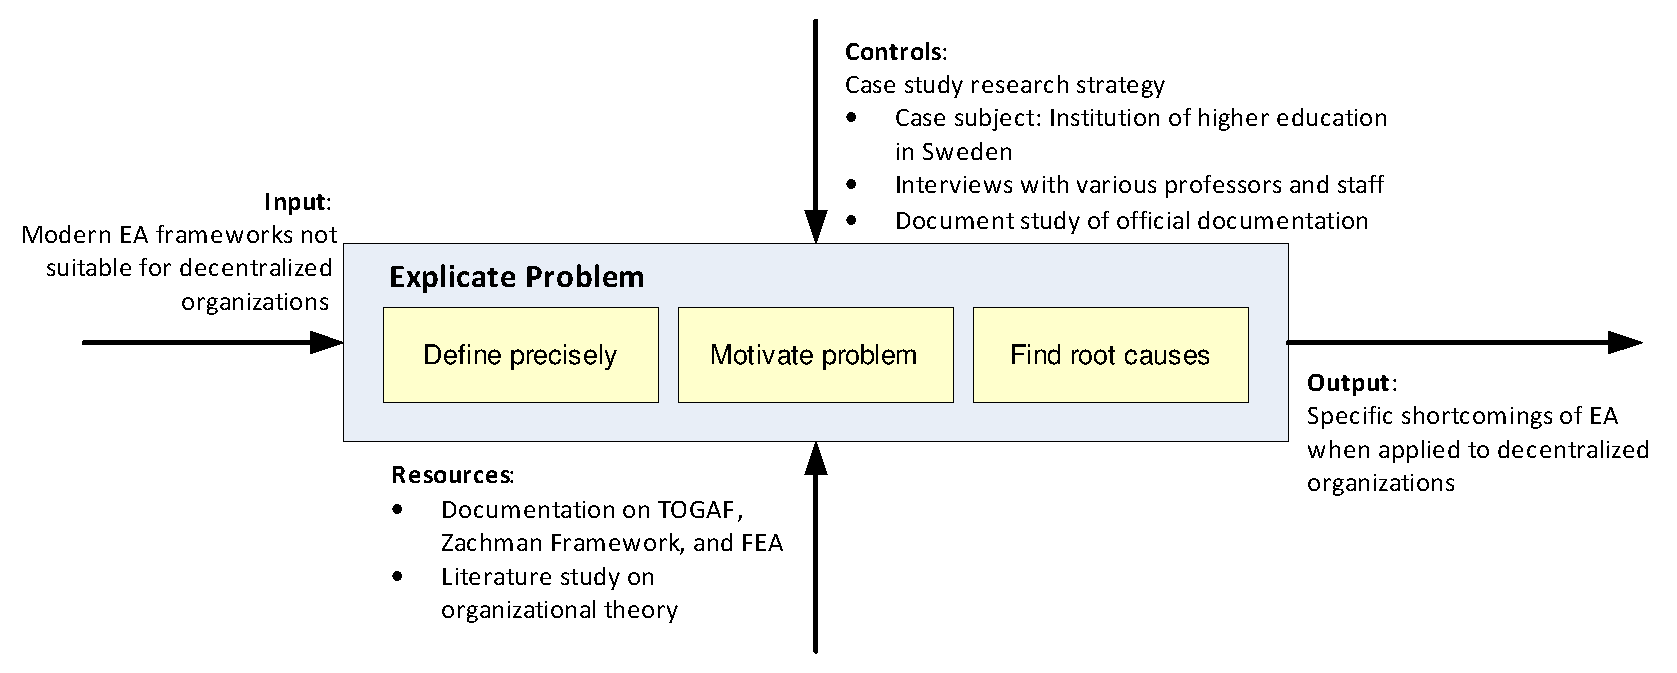
\includegraphics[scale=0.5]{method_problem}
\caption{Explicate problem activity}
\label{fig:method_problem}
\end{figure}

\subsubsection*{Outline artifact and define requirements}

Figure \ref{fig:method_outline} outlines the major components of this activity:
\begin{description}
  \item[Sub-activities] Outline Artifact and Define Requirements~\cite[Ch. 6]{johannessonPerjons2012}
  \item[Input] Set of specific shortcomings of modern EA frameworks when applied to decentralized organizations
  \item[Resources] Literature study on centralization/decentralization in  organizations
  \item[Controls] Case study research strategy
  \item[Output] Requirements for part of a decentralized EA
\end{description}

\paragraph{Iteration \#2}

In the first sub-activity Outline Artifact, the type of artifacts being developed is specified. 

In the second sub-activity, Define Requirements, the requirements for the developed artifact are elicited. This is based on the specific shortcomings of the case's EA, the specific shortcomings of EA frameworks, and on the literature study on centralization/decentralization in organizations.


\begin{figure}
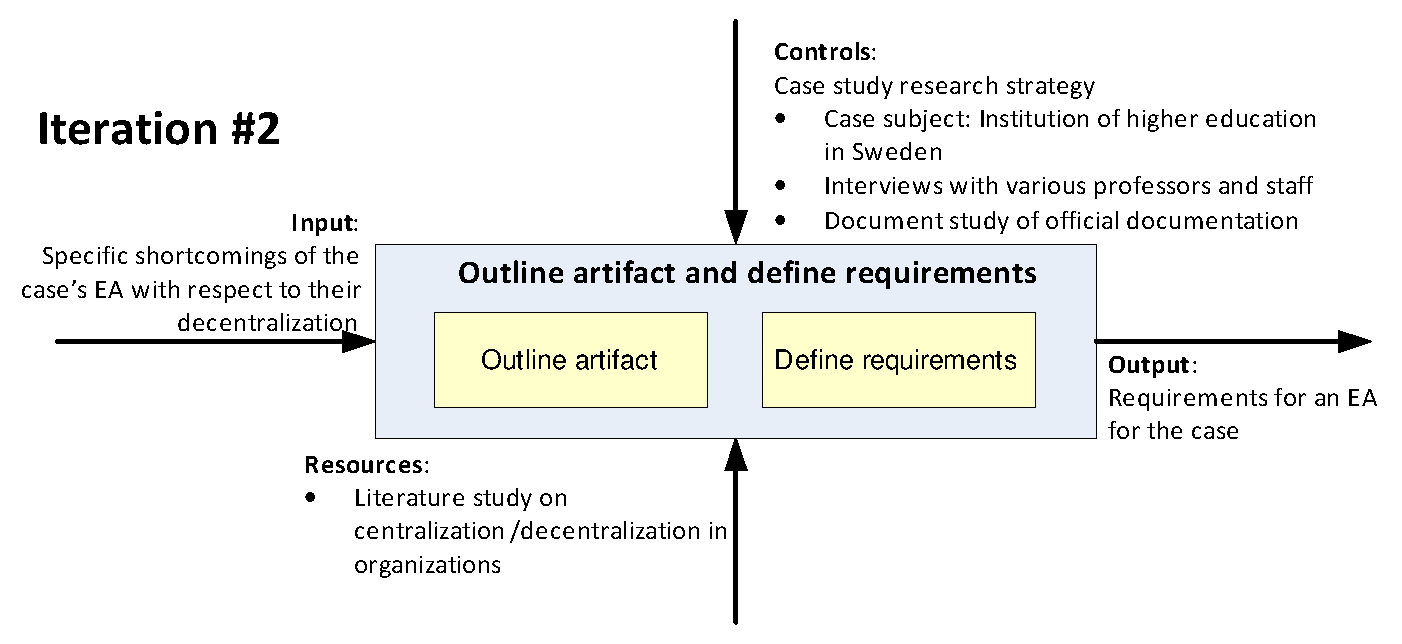
\includegraphics[scale=0.5]{method_outline}
\caption{Outline artifact and define requirements activity}
\label{fig:method_outline}
\end{figure}

\subsubsection*{Design and develop artifact}

Figure \ref{fig:method_design} outlines the major components of this activity:
\begin{description}
  \item[Sub-activities] Generate and Search and Select ~\cite[Ch. 7]{johannessonPerjons2012}
  \item[Input]  Requirements for a decentralized EA 
  \item[Resources] Literature study on peer-to-peer architectures
  \item[Controls] None
  \item[Output] Prototype of one artifact for one aspect of an EA framework for decentralized organizations 
\end{description}

\paragraph{Iteration \#1}

In this iteration, only the Generate sub-activity is performed. Here, a small number of different artifacts that could be potential solutions are outlined. The basis for these artifacts comes from a literature study on peer-to-peer architectures where principles relevant to EA are identified. Peer-to-peer architectures were chosen because they have offered solutions to decentralization in other domains (e.g. technical) and might therefore be able to provide solutions for the practice of EA. 

\paragraph{Iteration \#2}

In this iteration, one of the outlined solutions is selected and elaborated on to create a prototype of one artifact for an EA framework for decentralized organizations. This selection is based on its applicability to the case. 

\begin{figure}
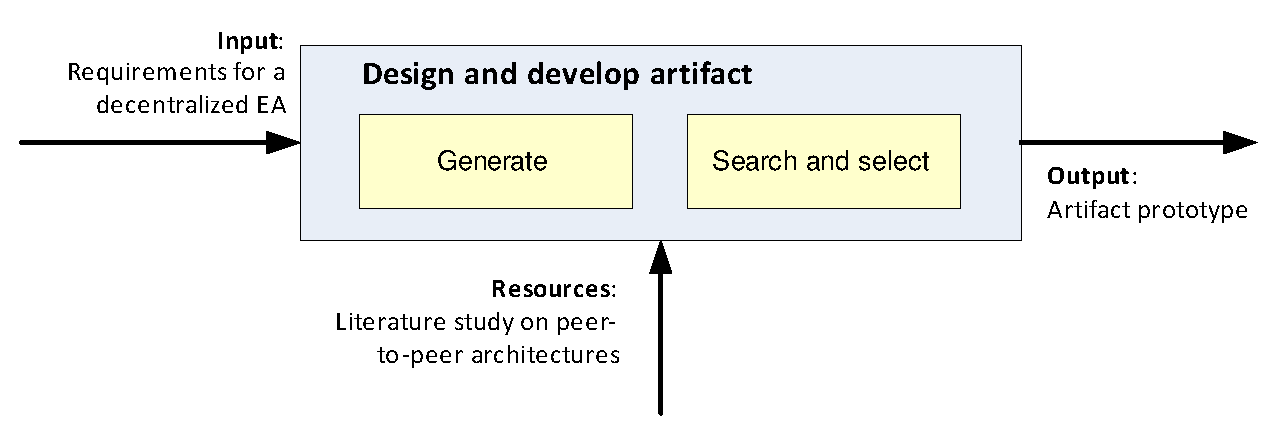
\includegraphics[scale=0.5]{method_design}
\caption{Design and develop artifact activity}
\label{fig:method_design}
\end{figure}
  
\subsubsection*{Demonstrate artifact}

Figure \ref{fig:method_demo} outlines the major components of this activity:
\begin{description}
  \item[Sub-activities]  Choose or Design Case and Apply Artifact~\cite[Ch. 8]{johannessonPerjons2012}
  \item[Input] Prototype of one artifact for one aspect of an EA framework for decentralized organizations
  \item[Resources]  Knowledge on the selected case (institution of higher education in Sweden)
  \item[Controls]  A case study research strategy that will make use of interviews and a document study
  \item[Output] Proof-of-concept artifact for one part of an EA framework prototype
\end{description}

\paragraph{Iteration \#1}

This activity is not performed in the first iteration. 

\paragraph{Iteration \#2}
For the Choose or Design Case sub-activity, an institution of higher education in Sweden has been selected. Details on the case are described in \ref{sec:case}.

In the Apply Artifact sub-activity, the artifact is applied to the case by creating a to-be architecture for the relevant aspect of the case. This to-be architecture is the proof-of-concept artifact for one part of an EA framework prototype.

\begin{figure}
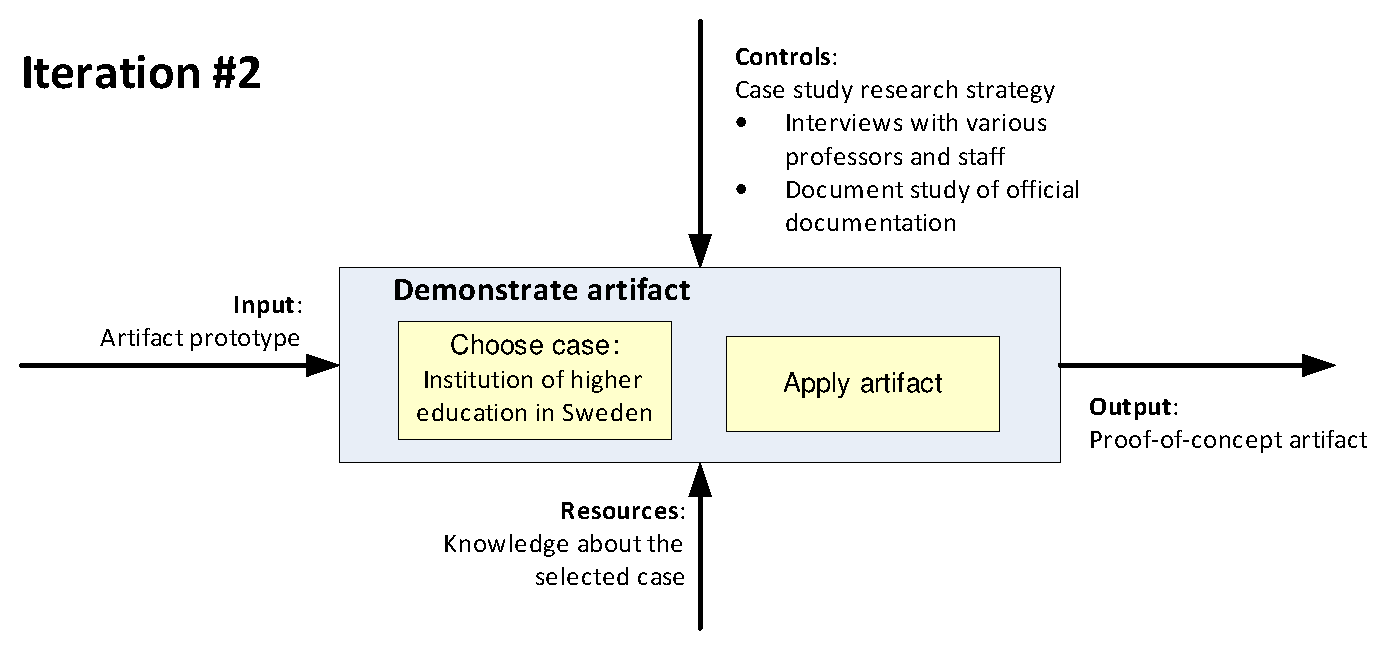
\includegraphics[scale=0.5]{method_demo}
\caption{Demonstrate artifact activity}
\label{fig:method_demo}
\end{figure}

\subsubsection*{Evaluate artifact}

Figure \ref{fig:method_evaluation} outlines the major components of this activity:
\begin{description}
  \item[Sub-activities] Choose Evaluation Strategy and Carry Out Evaluation~\cite[Ch. 8]{johannessonPerjons2012}
  \item[Input] Proof-of-concept artifact for one part of an EA framework prototype
  \item[Resources]  Knowledge on the selected case (institution of higher education in Sweden)
  \item[Output] An evaluated artifact
\end{description}

\paragraph{Iteration \#1}

This activity is not performed in the first iteration. 

\paragraph{Iteration \#2}

In the Choose Evaluation Strategy sub-activity, an \textit{ex ante} evaluation strategy is followed; this means that ``the artifact is evaluated without being used''~\cite[Ch. 9.1]{johannessonPerjons2012}. Johanneson and Perjons suggest interviews with experts for this sub-activity, however their are no experts available in the case organization, therefore an argumentative approach is instead being followed. The chosen evaluation strategy must be able to show that the artifact solves the explicated problem and fulfils the defined requirements.

In the Carry Out Evaluation sub-activity, the decided upon evaluation strategy is carried out to create the output for this activity; an evaluated artifact. 

\begin{figure}
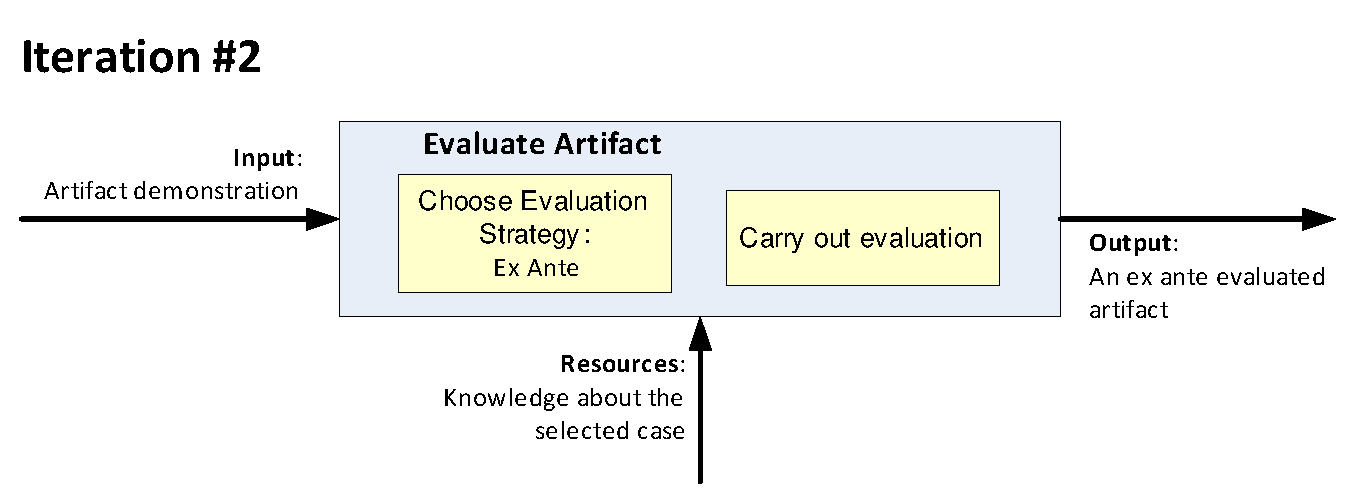
\includegraphics[scale=0.5]{method_evaluation}
\caption{Evaluate artifact activity}
\label{fig:method_eval}
\end{figure}

\section{Ethical Considerations}

As the proof-of-concept does not involve any actual implementation, the ethical considerations for this research project are minimal and only involve withholding the identity of the case institution. 

    
    %Part 4 - Results
    
    \chapter{Results}
    \label{chap:results}  
    
    \section{Explicate Problem}    
    \label{sec:problem}
    %\input{}

    %Part 5 - Discussion and Conclusion

% Move to PROBLEM MOTIVATION
%Enterprise Architecture is a discipline  that allows an organization to construct and evolve its IT according to its needs. It provides a methodology and sets up a framework for assessing the current state of IT (architecture As-Is), for agreeing upon and communicating its future state (architecture To-Be), for planning, and for carrying out this transformation. Though, it is important that  EA methodology and structures acknowledge progressive decentralization and help the organization to tackle the challenges related to it.    
    
    
%    Thus, there is a need for better process management
%[17, 23] and for more integration within decentralized
%and modular individual enterprises (e.g. most discrete
%parts manufacturing companies) as well as among
%networks of enterprises belonging to the same group or
%cooperating on large collaborative projects (e.g.
%Daimler-Chrysler or the AIRBUS Consortium).
    
    \section{Outline Artifact and Define Requirements}
    \label{sec:outline}
    %\input{}    
    
    \section{Design and Develop Artifact}
    \label{sec:design}
    %\input{}
    
    \section{Demonstrate Artifact}
    \label{sec:demo}
    %\input{}    
    
    \chapter{Conclusion and Discussion}
    
    
    

    \backmatter
    % References
    % No restriction is set to the reference styles
    % Save your references in References.bib

    % \urlstyle{same}         
    % Uncomment the line above to make urls have the same font and
    % size as the surrounding text. 

%    from paper    
%    \renewcommand{\baselinestretch}{0.98}
%    \bibliographystyle{IEEEtran}
%    {\small
%    \bibliography{biblioDecentralizedEA}
%    }
%    \renewcommand{\baselinestretch}{1}

%    from SU
%    \bibliographystyle{plain}
%    \bibliography{biblioDecentralizedEA}


    \bibliographystyle{IEEEtran}
    \bibliography{biblioDecentralizedEA}

%    \finalpageDSV

\end{document}